\section{Platforma mobilna (Java ME)}
\label{sec:javame-app}
Jednym z elementów rozwoju możliwości robota mobilnego Dark Explorer było
stworzenie aplikacji zarządzającej na urządzenia przenośne. W ramach tego zadania
stworzono aplikację działającą na platformie Java ME\footnote{Java ME - Java
Micro Edition}. Platforma ta jest dedykowana dla aplikacji tworzonych na
urządzenia mobilne o bardzo ograniczonych zasobach, takich jak telefony
komórkowe.

W związku z niską wydajnością procesorów oraz małą ilością pamięci w telefonach
komórkowych Java ME posiada ograniczony w stosunku do Java SE\footnote{Java SE -
Java Standard Edition, wersja platformy Java na komputery stacjonarne} zbiór klas
nazywanych konfiguracją. W Java ME wyróżniamy twa typy konfiguracji:
CDC\footnote{CDC -- Connected Device Configuration} dla urządzeń o lepszych
parametrach (smartfony) oraz CLDC\footnote{CLDC -- Connected Limited Device
Configuration} dla urządzeń o słabych parametrach (proste telefony komórkowe). W
tej pracy wykorzystana została konfiguracja CLDC.

Konfiguracje Java ME są uzupełniane przez profile MIDP\footnote{MIDP -- Mobile
Information Device Profile} które dodają swoje własne klasy do klas istniejących
w konfiguracji. Klasy te zapewniają wykonywanie odpowiednich zadań na konkretnych
elementach urządzenia mobilnego. Aplikacje wykorzystujące MIDP nazywane są
MIDletami i są uruchamiane w środowisku KVM\footnote{KVM - K Virtual Machine}.

K Virtual Machine jest niczym innym jak wirtualną maszyną Java opracowaną dla
konfiguracji CLDC. Jest ona bardzo ograniczona przez co posiada mniejsze
wymagania sprzętowe w porównaniu ze swoimi odpowiednikami z komputerów klasy PC.
Każdy producent urządzeń mobilnych musi zadbać o własną implementację maszyny
wirtualnej na której będą uruchamiane MIDlety.

\subsection{Narzędzia programistyczne}
Do rozwoju oprogramowania na platformę mobilną Java ME niezbędne jest
przygotowanie odpowiedniego środowiska programistycznego. Na potrzeby tej pracy
zostało wykorzystane zintegrowane środowisko programistyczne Eclipse, którego
krótki opis instalacji i konfiguracji znajduje się w rozdziale
\ref{sec:eclipse-inst-conf}. Dużym ułatwieniem pracy jest zainstalowanie Mobile
Tools for Java, dodatku do aplikacji Eclipse. Pozwala on na łatwe zarządzanie
projektem oprogramowania na urządzenie mobilne. Przykładowe okno, przedstawiające
przegląd właściwości projektu, wyświetlone dzięki temu dodatkowi przedstawia rys.
\ref{fig:MobTools4J}. Informacje na temat instalacji i konfiguracji dodatku można
znaleźć na stronie: \url{http://www.eclipse.org/mtj/}.

\begin{figure}[!ht]
 \centering 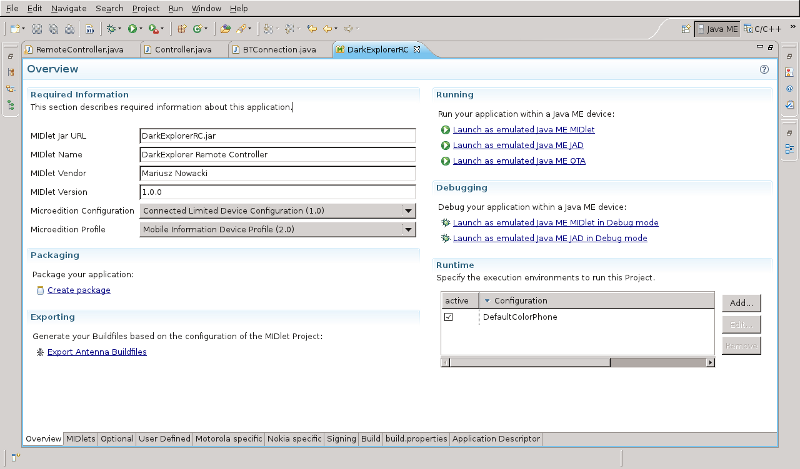
\includegraphics[height=75mm]{../images/ch05/mobile_tools_4_j.png}
 \caption{Okno konfigurujące właściwości projektu Java ME.}
 \label{fig:MobTools4J}
\end{figure}

Najważniejszym elementem przygotowywanego środowiska jest J2ME Wireless Toolkit
czyli zestaw narzędzi do tworzenia oprogramowania na urządzenia mobilne w którego
skład wchodzi między innymi emulator telefonu komórkowego. W chwili pisania tej
pracy istniał nowszy zestaw narzędzi o nazwie Java Platform Micro Edition
Software Development Kit 3.0. Nie spełniał jednak wymagań tej pracy co do
multiplatformowości gdyż jest dostępny w wersji tylko dla systemów Windows. Po
pobraniu Java Wireless Toolkit ze strony
\url{http://www.oracle.com/technetwork/java/download-135801.html} oraz jego
instalacji można przejść do projektowania aplikacji mobilnej.

\subsection{Aplikacja mobilna}
W ramach tej pracy magisterskiej napisano aplikację działającą na telefonach
komórkowych z zainstalowaną maszyną wirtualną Java. Została ona zaprojektowana w
taki sposób aby funkcjonalnością przypominać pilota do zdalnego sterowania.
Aplikacja korzysta z biblioteki zarządzającej robotem opisanej w rozdziale
\ref{subsec:sdk-java}. Rysunki \textcolor{red}{TODO: zrzut ekranu z aplikacji
mobilnej} przedstawiają uruchomioną aplikację mobilną.

Procedura instalacja aplikacji jest uzależniona od modelu telefonu na którym
będzie wykorzystywana. Należy pamiętać o włączeniu modułu bluetooth przed
uruchomieniem aplikacji sterującej robotem. Po przygotowaniu telefonu można
zacząć korzystać z aplikacji mobilnej.